\subsection{Introduction}


Transcranial electrical and magnetic stimulation  (TES and TMS, respectively) have been increasingly used in studies over the last decades and have been found to
alter and enhance cognitive processes
\supercite{Walsh2000,Lage2016,Paulus2016}. Furthermore, deep brain stimulation (DBS) has shown remarkable results in the treatment of tremor symptoms in 
Parkinsons disease \supercite{Collomb-Clerc2015} and also great potential 
in the treatment of psychiatric disorder such as obsessive-compulsive disorder \supercite{Alonso2015}.
However, despite this growing success in clinical settings, a principled understanding of the effects of stimulation on the dynamical processes in the brain 
is still lacking and, hence, stimulation parameters and target areas are currently not being optimized in a systematic fashion.    

Therefore, Muldoon et al. \supercite{Muldoon2016} develop a framework to explore the effects of targeted transcranial or deep brain stimulation on overall 
brain dynamics. In their framework they use data-driven computational model based on subject-specific structural connectivity and a nonlinear model of regional
brain activity (the so-called Wilson-Cowan model \supercite{Wilson1972}). Furthermore, they demonstrate that structure-based measures from linear network control theory 
can predict the functional effect of targeted stimulation.

In this work, we present an implementation of the modelling framework from Muldoon et al. \supercite{Muldoon2016} writtem im pure Python, where we exchanged
the model of regional brain activity to a simpler, phenomenological model, the FitzHugh Nagumo model \supercite{FitzHugh1961}. We report a \textit{partial/full(?)} 
replication of their results.
\subsection{Methods}

\paragraph{Overview}
The original model is, to the best of our knowledge, not publicly available. Therefore, this reimplementation is purely based on the description in the original
article and its supplementary material. The reimplementation is written in Python (2.7/3.6? tested with the other?). 

We have made two major changes compared to the original article: First, because we did not have access to the DTI data set used in the article, we used publicly
available DTI data form the Human Connectome Project \supercite{}. Second, we replaced the Wilson-Cowan model \supercite{Wilson1972} by the simpler and 
more efficient FithHugh Nagumo model \supercite{FitzHugh1961}. Both changes will be explained in more detail in the following sections and commented on in the 
discussion.
\paragraph{Structural connectivity}
As explained above, we did not have access to the diffusion tensor imaging (DTI) data form the original article. We thus used DTI data from 10 healthy
subjects (mean+std age and gender distribution; possibly even more demographic info \textbf{\textit{Nico!}}) from the publicly available HCP1200 data set of the
Human Connectome Project (\textit{link}).

\begin{itemize}
 \item 
  Acquisition information from HCP
 \item
  Preprocessing: software tool, steps and parameters  \textbf{\textit{Nico! Maybe Cristiana?}}
 \item
  Structural connectivity matrices: Parcellation scheme, thresholding, normalization \textbf{\textit{Nico!}}
\end{itemize}

\textit{Do we have repeated scans of the same individuals? If not, we cannot look at Reproducibility and the within subject
variability (see Figure 2 d). Not a big problem, but should then be mentioned here!}

\paragraph{Model of regional brain dynamics}
The second part that is necessary to model the dynamic evolution of brain activity across the entire brain, is a computational model of the
regional brain dynamics. In the original article, Muldoon et al. \supercite{Muldoon2016} use the Wilson-Cowan model \supercite{Wilson1972}. The Wilson-Cowan model
describes the interaction between a local excitatory and a local inhibitory neural population by two coupled differential equations. However, due to the different
parameters describing the coupling of the populations and the synaptic interactions, the Wilson-Cowan model has more then ten free parameters and, thus,
a high degree of unconstrained variability. Therefore, we opted to exchange the Wilson-Cowan model by the FitzHugh Nagumo (FHN) model \supercite{FitzHugh1961}, which
only has four (\textit{correct?}\textbf{\textit{Nico!}}) free parameters and, additionally, is computationally slightly more efficient than the Wilson-Cowan model.

The FHN is given by...\textit{  FHN equations and parameters (plus explanation)} \textbf{\textit{Nico!}}


Importantly, the FHN model displays the same three dynamical states depending on the strength of its input than the Wilson-Cowan model (see Figure \ref{fig:FHN}): 
First, for weak input the FHN resides in a stable fixed point with low activity. Second, for stronger inputs the FHN then transitions into an oscillatory
regime and, last, for even stronger inputs it then settles into a stable fixed point again, however, this time with a very high activity.

\begin{figure}
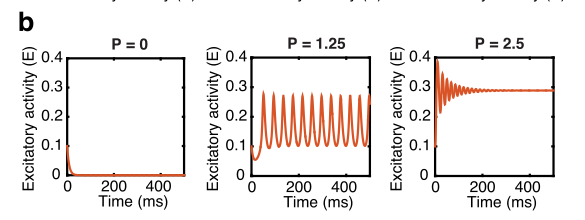
\includegraphics{Figures/placeholder}
 \caption{ 3 states of the FitzHugh Nagumo (and comparison to the Wilson-Cowan?) \textbf{\textit{Nico!}}}
 \label{fig:FHN}
\end{figure}









\paragraph{Individual oscillatory transition paramters}

\paragraph{Inter- and intra-subject reproducibility and variability}
\textit{depends on whether we have repeated scans of same individuals or not}
\paragraph{Linear network control theory}

\paragraph{Functional and structural effect, and fractional activation}


\subsection{Reproduction of experiments}

\begin{itemize}
 \item 
  Replicate Figure 2 (c) and (d) 
  and for c) our box plots for all subjects, and d) bar plots with our data
  
 \item
  Replicate Figure 3 

 \item
  Replicate Figure 4 c) 
  
 \item
  Replicate Figure 5 a)-d)
  
 \item
  Replicate Figure 6 (?)
\end{itemize}

I don't think we need to replicate Figure 7 (Structure-function landscape)

\subsection{Reimplementation}

\begin{itemize}
 \item 
  Details on the new implementation (packages/dependencies, other stuff?, maybe just a paragraph in the methods section) 
\end{itemize}

 




\subsection{Discussion}

\begin{itemize}
 \item 
  Main similarities and differences between our and original results. Replication: full, partial or not at all?
\end{itemize}
